%%%%%%%%%%%%%%%%%%%%%%%%%%%%%%%%%%%%%%%%%
% University/School Laboratory Report
% LaTeX Template
% Version 3.1 (25/3/14)
%
% This template has been downloaded from:
% http://www.LaTeXTemplates.com
%
% Original author:
% Linux and Unix Users Group at Virginia Tech Wiki 
% (https://vtluug.org/wiki/Example_LaTeX_chem_lab_report)
%
% License:
% CC BY-NC-SA 3.0 (http://creativecommons.org/licenses/by-nc-sa/3.0/)
%
%%%%%%%%%%%%%%%%%%%%%%%%%%%%%%%%%%%%%%%%%

%----------------------------------------------------------------------------------------
%	PACKAGES AND DOCUMENT CONFIGURATIONS
%----------------------------------------------------------------------------------------

\documentclass{article}

\usepackage{graphicx} % Required for the inclusion of images
\usepackage{amsmath} % Required for some math elements 
\usepackage{cite}
\usepackage{subcaption} %Required to group figures
%\usepackage{float}

\setlength\parindent{0pt} % Removes all indentation from paragraphs

%\usepackage{times} % Uncomment to use the Times New Roman font

%----------------------------------------------------------------------------------------
%	DOCUMENT INFORMATION
%----------------------------------------------------------------------------------------

\title{Lab 5\\ Baseband PAM\\ EE 445S} % Title

\author{Enoc Balderas\\
        \and
        Daniel Diamont\\} % Author name

\date{\today} % Date for the report

\begin{document}

\maketitle % Insert the title, author and date

\begin{center}
\begin{tabular}{l r}
Date Performed: & April 22, 2019 \\ % Date the experiment was performed
Instructor: & Professor Evans % Instructor/supervisor
\end{tabular}
\end{center}

% If you wish to include an abstract, uncomment the lines below
% \begin{abstract}
% Abstract text
% \end{abstract}

%----------------------------------------------------------------------------------------
%	SECTION 1
%----------------------------------------------------------------------------------------

\section{Introduction}

\subsection{Pulse Shaping}

%----------------------------------------------------------------------------------------
%	SECTION 2
%----------------------------------------------------------------------------------------

\section{Methods}

\subsection{Pulse Shaping}

%----------------------------------------------------------------------------------------
%	SECTION 3
%----------------------------------------------------------------------------------------

\section{Results}

\subsection{QAM Modulation}

\begin{figure}[h]
  \begin{center}
    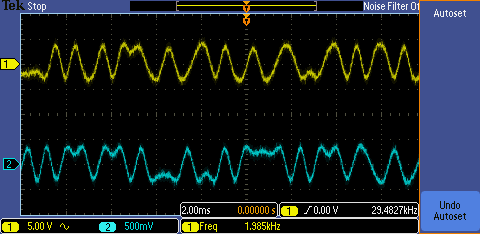
\includegraphics[width=0.65\textwidth]{img/task_a_oscilloscope.png}
    \caption{In-phase and Quadrature component.}
  \end{center}
\end{figure}

\begin{figure}[h]
  \begin{center}
    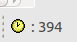
\includegraphics[width=0.65\textwidth]{img/task_a_profile.png}
    \caption{In-phase and Quadrature component.}
  \end{center}
\end{figure}

\begin{figure}[h]
  \begin{center}
    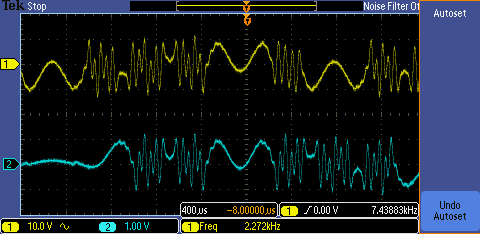
\includegraphics[width=0.65\textwidth]{img/task_b_oscilloscope.png}
    \caption{In-phase and Quadrature component of PN sequence.}
  \end{center}
\end{figure}

\begin{figure}[h]
  \begin{center}
    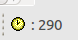
\includegraphics[width=0.65\textwidth]{img/task_b_profile.png}
    \caption{In-phase and Quadrature component of PN sequence.}
  \end{center}
\end{figure}

\begin{figure}[h]
  \begin{center}
    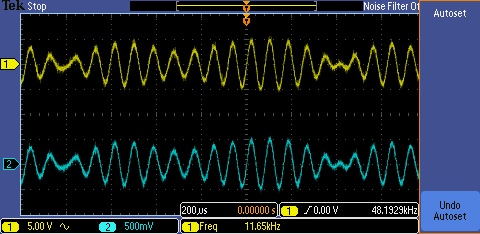
\includegraphics[width=0.65\textwidth]{img/task_c_oscilloscope.png}
    \caption{In-phase and Quadrature component of PN sequence.}
  \end{center}
\end{figure}

\begin{figure}[h]
  \begin{center}
    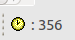
\includegraphics[width=0.65\textwidth]{img/task_c_profile.png}
    \caption{In-phase and Quadrature component of PN sequence.}
  \end{center}
\end{figure}

\begin{figure}[h]
  \begin{center}
    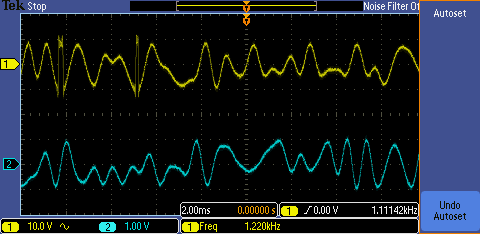
\includegraphics[width=0.65\textwidth]{img/task_d_oscilloscope.png}
    \caption{In-phase and Quadrature component of PN sequence.}
  \end{center}
\end{figure}

\begin{figure}[h]
  \begin{center}
    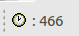
\includegraphics[width=0.65\textwidth]{img/task_d_profile.png}
    \caption{In-phase and Quadrature component of PN sequence.}
  \end{center}
\end{figure}

\textbf{Code:}

\begin{verbatim}

	// left (quadrature), right (in-phase)
	const float QPSK_LUT[16][2] = {
	{     -3 * QPSK_SCALE,  -3 * QPSK_SCALE}, /* QPSK_LUT[0]  */
	{     -3 * QPSK_SCALE, -1 * QPSK_SCALE}, /* QPSK_LUT[1]  */
	{    -3 * QPSK_SCALE,  3 * QPSK_SCALE}, /* QPSK_LUT[2]  */
	{    -3 * QPSK_SCALE,  1 * QPSK_SCALE}, /* QPSK_LUT[3]  */
	{    -1 * QPSK_SCALE, -3 * QPSK_SCALE}, /* QPSK_LUT[4]  */
	{    -1 * QPSK_SCALE, -1 * QPSK_SCALE}, /* QPSK_LUT[5]  */
	{    -1 * QPSK_SCALE,  3 * QPSK_SCALE}, /* QPSK_LUT[6]  */
	{    -1 * QPSK_SCALE,  1 * QPSK_SCALE}, /* QPSK_LUT[7]  */
	{     3 * QPSK_SCALE, -3 * QPSK_SCALE}, /* QPSK_LUT[8]  */
	{     3 * QPSK_SCALE, -1 * QPSK_SCALE}, /* QPSK_LUT[9]  */
	{     3 * QPSK_SCALE,  3 * QPSK_SCALE}, /* QPSK_LUT[10]  */
	{     3 * QPSK_SCALE,  1 * QPSK_SCALE}, /* QPSK_LUT[11]  */
	{     1 * QPSK_SCALE, -3 * QPSK_SCALE}, /* QPSK_LUT[12]  */
	{     1 * QPSK_SCALE, -1 * QPSK_SCALE}, /* QPSK_LUT[13]  */
	{     1 * QPSK_SCALE,  3 * QPSK_SCALE}, /* QPSK_LUT[14]  */
	{     1 * QPSK_SCALE, -1 * QPSK_SCALE}, /* QPSK_LUT[15]  */
	};

	/****************************************************************/
	// I added my impulse modulated QPSK routine here
	if (counter == 0) {
		symbol = rand() & 0xF;

		xI[0]  = QPSK_LUT[symbol][RIGHT];  
		xQ[0]  = QPSK_LUT[symbol][ LEFT];   
	}

	// perform impulse modulation based on the FIR filter, B[N]
	yI = 0;
	yQ = 0;

	for (i = 0; i < span; i++) {
		// perform the "I" dot-product
		yI += xI[i]*pulse[counter + samplesPerSymbol*i];	

		// perform the "Q" dot-product
		yQ += xQ[i]*pulse[counter + samplesPerSymbol*i];	
	}

	if (counter >= (samplesPerSymbol - 1)) {
		counter = -1; 

		/* shift xI[] and xQ[] in preparation to receive the next input */
		for (i = 5; i > 0; i--) {
			// setup xI[] for the next input value
			xI[i] = xI[i-1];  

			// setup xQ[] for the next input value
			xQ[i] = xQ[i-1];  
		}
	}

	counter++;

	output = output_gain*(yI*cosine[counter & 3] - yQ*sine[counter & 3]);
\end{verbatim}

\begin{figure}[h]
  \begin{center}
    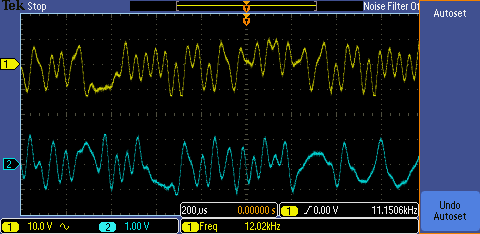
\includegraphics[width=0.65\textwidth]{img/task_e_oscilloscope.png}
    \caption{In-phase and Quadrature component of PN sequence.}
  \end{center}
\end{figure}

\begin{figure}[h]
  \begin{center}
    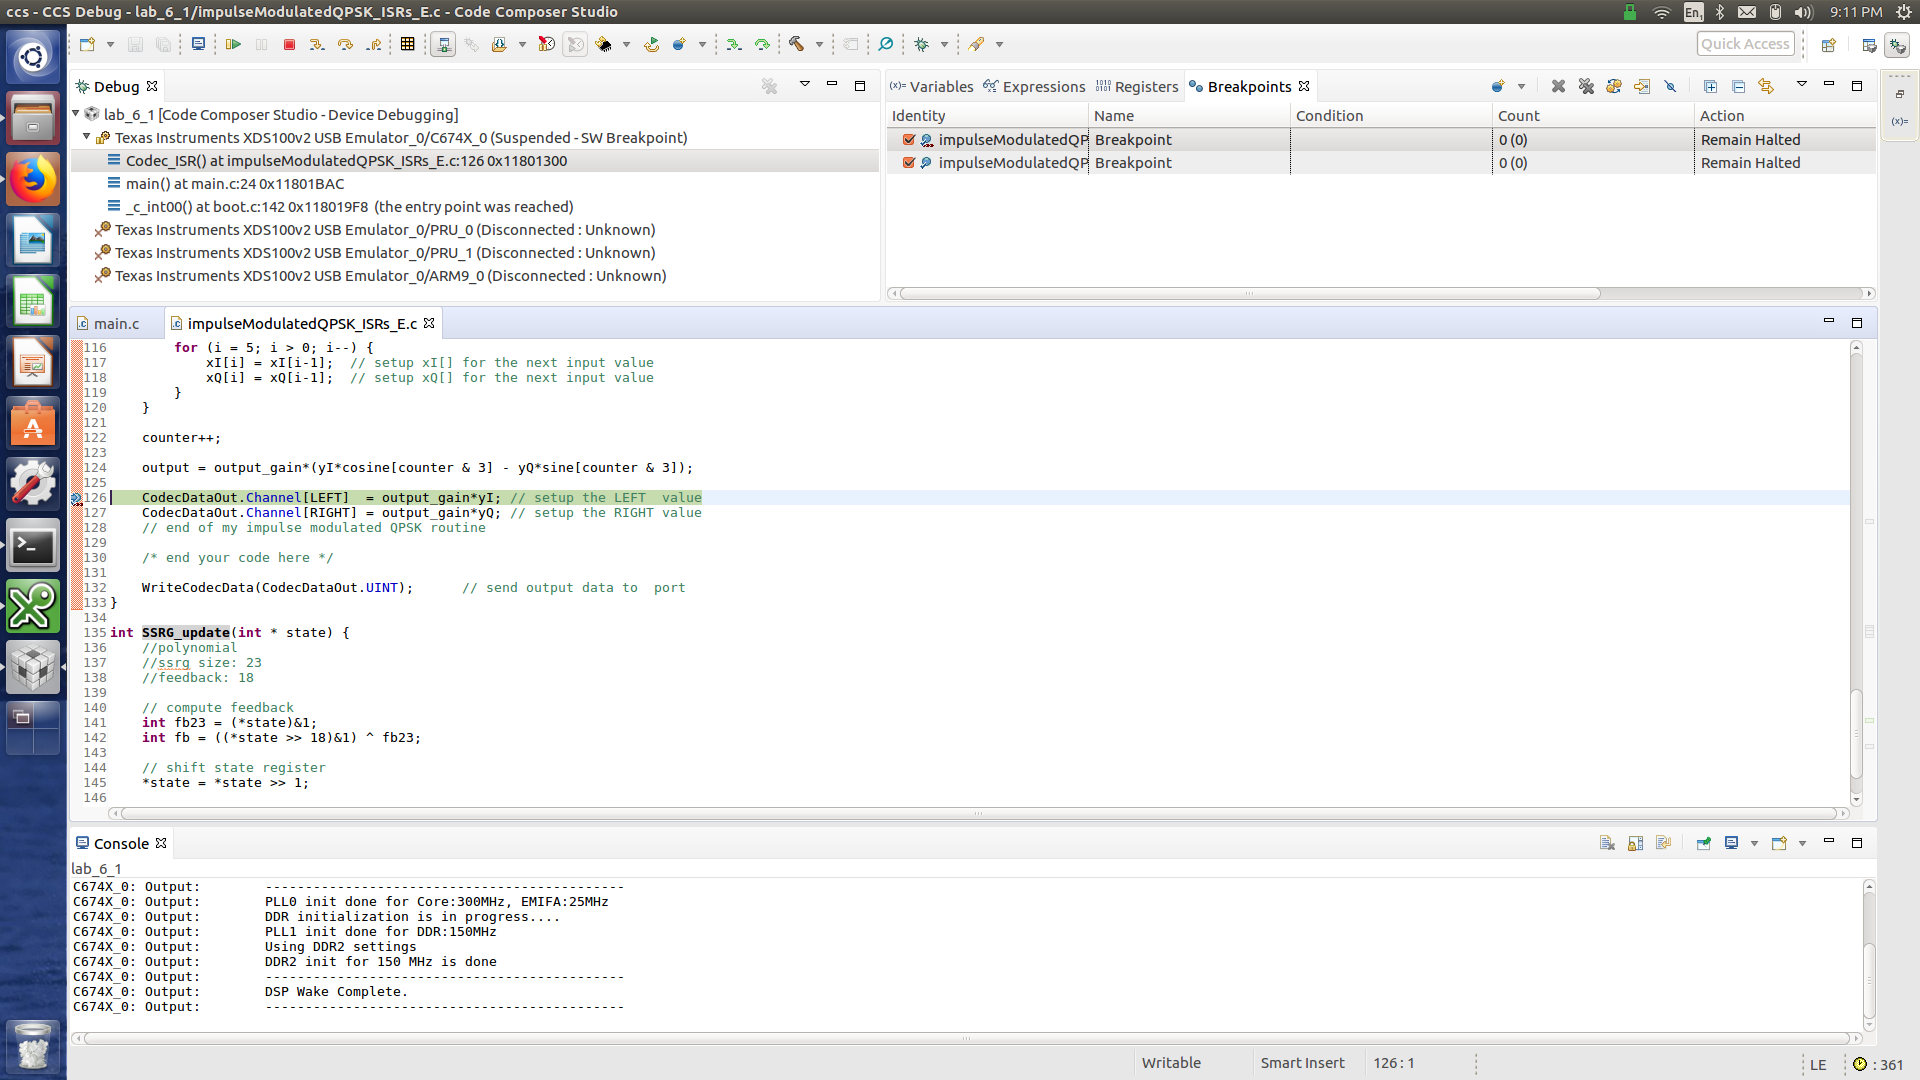
\includegraphics[width=0.65\textwidth]{img/task_e_profile.png}
    \caption{In-phase and Quadrature component of PN sequence.}
  \end{center}
\end{figure}

\textbf{Code:}

\begin{verbatim}

	// left (quadrature), right (in-phase)
	const float QPSK_LUT[16][2] = {
	{     -3 * QPSK_SCALE,  -3 * QPSK_SCALE}, /* QPSK_LUT[0]  */
	{     -3 * QPSK_SCALE, -1 * QPSK_SCALE}, /* QPSK_LUT[1]  */
	{    -3 * QPSK_SCALE,  3 * QPSK_SCALE}, /* QPSK_LUT[2]  */
	{    -3 * QPSK_SCALE,  1 * QPSK_SCALE}, /* QPSK_LUT[3]  */
	{    -1 * QPSK_SCALE, -3 * QPSK_SCALE}, /* QPSK_LUT[4]  */
	{    -1 * QPSK_SCALE, -1 * QPSK_SCALE}, /* QPSK_LUT[5]  */
	{    -1 * QPSK_SCALE,  3 * QPSK_SCALE}, /* QPSK_LUT[6]  */
	{    -1 * QPSK_SCALE,  1 * QPSK_SCALE}, /* QPSK_LUT[7]  */
	{     3 * QPSK_SCALE, -3 * QPSK_SCALE}, /* QPSK_LUT[8]  */
	{     3 * QPSK_SCALE, -1 * QPSK_SCALE}, /* QPSK_LUT[9]  */
	{     3 * QPSK_SCALE,  3 * QPSK_SCALE}, /* QPSK_LUT[10]  */
	{     3 * QPSK_SCALE,  1 * QPSK_SCALE}, /* QPSK_LUT[11]  */
	{     1 * QPSK_SCALE, -3 * QPSK_SCALE}, /* QPSK_LUT[12]  */
	{     1 * QPSK_SCALE, -1 * QPSK_SCALE}, /* QPSK_LUT[13]  */
	{     1 * QPSK_SCALE,  3 * QPSK_SCALE}, /* QPSK_LUT[14]  */
	{     1 * QPSK_SCALE, -1 * QPSK_SCALE}, /* QPSK_LUT[15]  */
	};

	/****************************************************************/
	// I added my impulse modulated QPSK routine here
	if (counter == 0) {
		/* generate 2 random bits */
		symbol = SSRG_update(&SSRG_state); 
		symbol = (symbol << 1) + SSRG_update(&SSRG_state);
		symbol = (symbol << 1) + SSRG_update(&SSRG_state);
		symbol = (symbol << 1) + SSRG_update(&SSRG_state);

		xI[0]  = QPSK_LUT[symbol][RIGHT];  
		xQ[0]  = QPSK_LUT[symbol][ LEFT];   
	}

	// perform impulse modulation based on the FIR filter, B[N]
	yI = 0;
	yQ = 0;

	for (i = 0; i < span; i++) {
		// perform the "I" dot-product
		yI += xI[i]*pulse[counter + samplesPerSymbol*i];	

		// perform the "Q" dot-product
		yQ += xQ[i]*pulse[counter + samplesPerSymbol*i];	
	}

	if (counter >= (samplesPerSymbol - 1)) {
		counter = -1; 

		/* shift xI[] and xQ[] in preparation to receive the next input */
		for (i = 5; i > 0; i--) {
			// setup xI[] for the next input value
			xI[i] = xI[i-1];  

			// setup xQ[] for the next input value
			xQ[i] = xQ[i-1];  
		}
	}

	counter++;

	output = output_gain*(yI*cosine[counter & 3] - yQ*sine[counter & 3]);
\end{verbatim}

\clearpage
\pagebreak

\begin{figure}[h]
  \begin{center}
    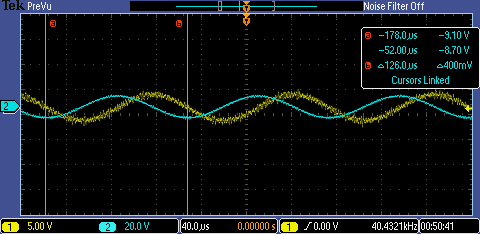
\includegraphics[width=0.65\textwidth]{img/task_2_b_oscilloscope.png}
    \caption{In-phase and Quadrature component of PN sequence.}
  \end{center}
\end{figure}

\begin{figure}[h]
  \begin{center}
    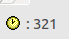
\includegraphics[width=0.65\textwidth]{img/task_2_b_profile.png}
    \caption{In-phase and Quadrature component of PN sequence.}
  \end{center}
\end{figure}

\begin{figure}[h]
  \begin{center}
    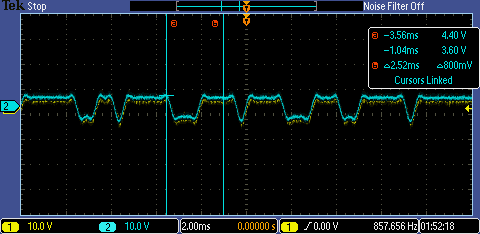
\includegraphics[width=0.65\textwidth]{img/task_2_c_oscilloscope.png}
    \caption{In-phase and Quadrature component of PN sequence.}
  \end{center}
\end{figure}

\begin{figure}[h]
  \begin{center}
    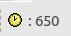
\includegraphics[width=0.65\textwidth]{img/task_2_c_profile.png}
    \caption{In-phase and Quadrature component of PN sequence.}
  \end{center}
\end{figure}

\begin{figure}[h]
  \begin{center}
    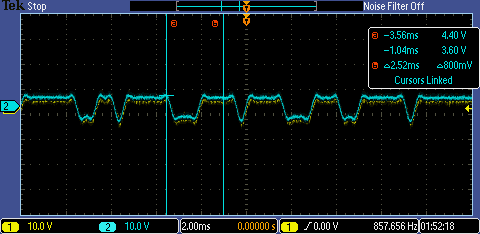
\includegraphics[width=0.65\textwidth]{img/task_2_c_oscilloscope.png}
    \caption{In-phase and Quadrature component of PN sequence.}
  \end{center}
\end{figure}

\begin{figure}[h]
  \begin{center}
    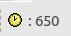
\includegraphics[width=0.65\textwidth]{img/task_2_c_profile.png}
    \caption{In-phase and Quadrature component of PN sequence.}
  \end{center}
\end{figure}

\begin{figure}[h]
  \begin{center}
    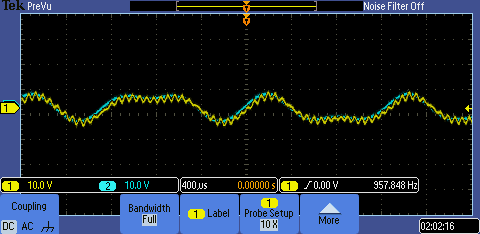
\includegraphics[width=0.65\textwidth]{img/task_2_d_delay.png}
    \caption{In-phase and Quadrature component of PN sequence.}
  \end{center}
\end{figure}

\begin{verbatim}
	// I added my impulse modulated QPSK routine here
	if (counter == 0) {
		/* generate 2 random bits */
		symbol = SSRG_update(&SSRG_state); 
		symbol = (symbol << 1) + SSRG_update(&SSRG_state);

		xI[0]  = QPSK_LUT[symbol][RIGHT];  
		xQ[0]  = QPSK_LUT[symbol][ LEFT];   
	}

	// perform impulse modulation based on the FIR filter, B[N]
	yI = 0;
	yQ = 0;

	for (i = 0; i < span; i++) {
		// perform the "I" dot-product
		yI += xI[i]*pulse[counter + samplesPerSymbol*i];	

		// perform the "Q" dot-product
		yQ += xQ[i]*pulse[counter + samplesPerSymbol*i];	
	}

	if (counter >= (samplesPerSymbol - 1)) {
		counter = -1; 

		/* shift xI[] and xQ[] in preparation to receive the next input */
		for (i = 5; i > 0; i--) {
			// setup xI[] for the next input value
			xI[i] = xI[i-1];  

			// setup xQ[] for the next input value
			xQ[i] = xQ[i-1];  
		}
	}

	counter++;
	carrier_index = (carrier_index + 1) % 6;

	output = output_gain*(yI*cosine[carrier_index] - yQ*sine[carrier_index]);
	// end of my impulse modulated QPSK routine

	//demodulate in-phase and quadrature
    float demod_inphase = 2*output*cosine[carrier_index];
    float demod_quad = -2*output*sine[carrier_index];

    //LPF
    biquad_x_inphase[0][0] = demod_inphase;
    biquad_x_quad[0][0] = demod_quad;

    float output_inphase = G[0] * biquad_inphase(0, biquad_x_inphase[0][0]);
    float output_quad = G[0] * biquad_quadrature(0, biquad_x_quad[0][0]);
\end{verbatim}

%----------------------------------------------------------------------------------------
%	SECTION 4
%----------------------------------------------------------------------------------------

\section{Discussion}

\subsection{Pulse Shaping}


%----------------------------------------------------------------------------------------
%	SECTION 5
%----------------------------------------------------------------------------------------

\section{Answers to questions}

\begin{enumerate}
  \begin{item}
		How could pulse shaping be implemented using only a single "filter" (not a bank of filters). Practically, why would this be undesirable?

  \textbf{Answer:}
		Pulse shaping could be implemented by convolving with a single FIR filter. This is undesirable because for baseband transmission we usually take our symbol amplitude vector and upsample (by some fator L) to the DAC frequency before pulse shaping. Because of this upsampling, the amplitude vector contains a lot of extra zeros, which would cause (L - 1) multiplications by 0 for every original symbol amplitude. By using a filter bank, we avoid these
		fruitless multiplications by 0, and obtain a factor of L performance improvement.
  \end{item}

  \begin{item}
		In the clock recovery system, discuss the need for a Prefiltering. For a symbol rate of 2 kHz, what would be the output if the prefilter attenuated all frequencies greater than 900 Hz? Would it be possible to recover the transmitter's symbol frequency (using the same squaring operation and post-filters as in the lab)? If not, give a short reason why.

  \textbf{Answer:}
		We prefilter to obtain a cosine with a center frequency of $fsym/2$ without high frequency noise. What we are interested in is capturing the phase ($\theta$) and frequency information (fsym) of the cosine to feed this into a Costas or Phase Lock Loop to determine the phase offset for sampling. Any other frequency content is unnecessary.

		If the output of the prefilter attenuated all frequencies greater than 900 Hz, we would not be able to recover the transmitter's symbol frequency because $fsym/2$ in this case equals 1 KHz, which would be attenuated by our hypothetical prefilter.
  \end{item}

\end{enumerate}

\end{document}
